\pgfplotsset{
    colormap={}{[5pt]
        rgb255(0pt)=(255, 255, 255);
        rgb255(1000pt)=(255, 111, 25)
    },
}

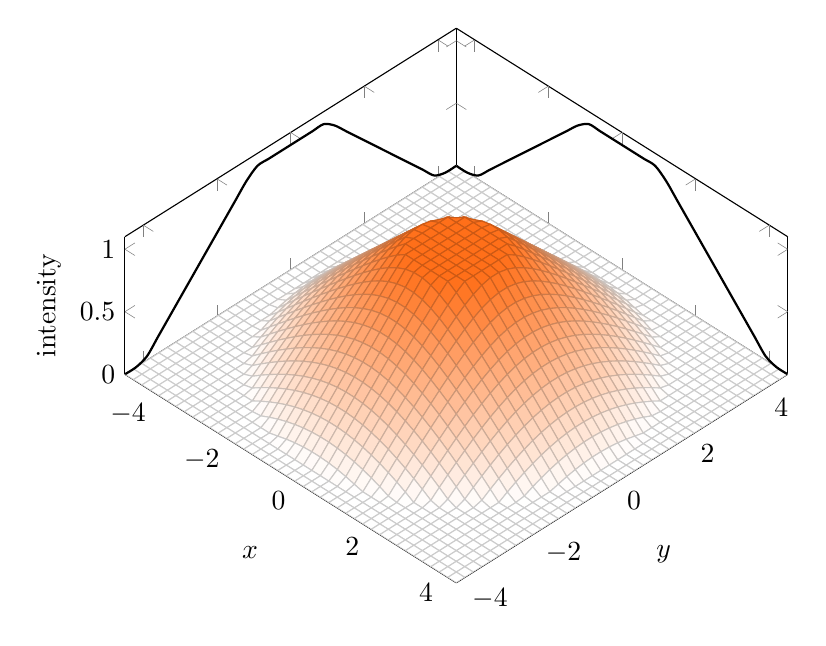
\begin{tikzpicture}[
    declare function={single(\x) = max(0,1 - (max(0,abs(x)-1)/3));},
    declare function={stench(\x,\y) = max(0,1-(max(0,((x^2)+(y^2))^(1/2)-1)/3));}]
\begin{axis}[
    width=10cm,
    view={45}{65},
    enlargelimits=false,
    domain=-4.5:4.5,
    y domain=-4.5:4.5,
    samples=40,
    xlabel=$x$,
    ylabel=$y$,
    zmax=1.1,
    zlabel={$\mathrm{intensity}$},
]
\addplot3 [surf] {stench(x,y)};
\addplot3 [domain=-4.5:4.5,samples=31, samples y=0, thick, smooth] (x,4.5,{single(x)});
\addplot3 [domain=-4.5:4.5,samples=31, samples y=0, thick, smooth] (-4.5,x,{single(x)});

\end{axis}
\end{tikzpicture}